\documentclass[a4paper,oneside,12pt]{article}
\usepackage[utf8]{inputenc}
\usepackage{dcolumn}
\usepackage[spanish]{babel}
\usepackage{graphicx}

\begin{document}

\pagenumbering{arabic}

\title{CRefactory}
\author{Baglivo Nicol\'as C\'esar \and Costa Federico Daniel \and Perera Nicanor Gonzalo \and Szeinfeld Matias Ezequiel \and Tarragona Juan Pablo}
\date{\today}
\maketitle

\tableofcontents

\newpage
\section{Organizaci\'on del documento}
Primero se dará una introduccion para poner en contexto al problema planteado por la c\'atedra junto con la  motivaci\'on para la realizaci\'on del trabajo. Se detallar\'an los objetivos del mismo así como tambi\'en la manera de trabajo del grupo.

Luego, se ir\'an detallando en orden de aparici\'on los problemas con los que nos fuimos enfrentando a lo largo de la cursada. Por cada uno de ellos se explicar\'a en que consiste junto a la soluci\'on planteada.
Mas adelante se listará un resumen de las minutas de cada reunión con la profesora.
Por \'ultimo se detallar\'an las conclusiones y el trabajo a futuro.

\section{Introducción}
El refactoring de c\'odigo es una técnica para la reestructuración del código existente de un producto de software, alterando su estructura interna sin cambiar su comportamiento externo con el objetivo de mejorar atributos no funcionales del software como pueden ser la legibilidad, la mantenibilidad o incluso la extensibidad del mismo. Existen una serie de t\'ecnicas bien conocidas de uso com\'un durante el proceso de refactoring de c\'odigo, CRefactory es un entorno de desarrollo que provee soporte para realizar de manera autom\'atica los aspectos mec\'anicos de dicho proceso mediante una interfaz gr\'afica.

Crefactory esta programado en Smalltalk dentro del entorno de desarrollo VisualWorks. La interfaz gr\'afica que posee la aplicaci\'on permite interactuar con c\'odigo C para facilitar dicha refactorizaci\'on. Provee la carga de archivos .c, y directorios con header files. as\'i como tambien configuraciones a descartar (macros y false conditions).  
Permite realizar refactoring de variables ( cambio de nombre, crear estructuras de las variables), de las estructuras (renombrar campos) y de funciones (renombrar las mismas).


\subsection{Motivaci\'on}
CRefactory funcionaba correctamente, pero estaba lejos de ser la herramienta ideal de trabajo, ya que su interfaz no era amigable con el usuario. En primer lugar, era muy poco pr\'actica la carga de archivos, ya que era necesario escribir el path de los archivos a mano, y no se pose\'ia ning\'un tipo de feedback para saber si se habia referenciado correctamente dicho archivo. Se vi\'o la necesidad de mejorar la manera en que se cargaraban los archivos.

En segundo lugar, la herramienta no era capaz de agregar false conditions o macros por medio de la interfaz, con lo cual se desaprovechaba  parte del poder de CRefactory. Era necesario de implementar esto de una manera amigable al usuario por medio de una interfaz gr\'afica.

En tercer lugar, no se entend\'ia que ocurr\'ia en caso de que se produzca una excepci\'on. Se necesitaba implementar una manera f\'acil y amigable para que se traten las mismas y as\'i detectar el error. Se necesitaba un mejor manejo de las excepciones y una interfaz para tratarlas.
Por ejemplo, si ocurr\'ia un error durante el parseo de un archivo, no mostraba el contenido del mismo y por ende no mostraba la l\'nea de c\'odigo que produjo el error. Por lo que tambi\'en fue necesario implementar highlighting para la detecci\'on de error en parseo.


\subsection{Objetivos}
Objetivos generales

Mejorar la experiencia del usuario al utilizar la herramienta haciendo \'enfasis en facilidad de uso, proveer feedback, manejo de excepciones, di\'alogo simple y natural, salidas evidentes, prevenci\'on de errores y ayudas.

Particularmente se desea mejorar la carga de archivos e include\_directories para que cumpla las siguientes condiciones: prevenci\'on de errores, facilidad de uso, simplicidad y menor sorpresa al usuario.

Implementar una interfaz que permita al usuario el manejo de macros y false conditions de una manera sencilla e intuitiva, de manera que pueda agregarlas o quitarlas a gusto.

Desarrollar una manera de visualizar la ocurrencia de errores y excepciones que sea adecuada, clara y funcional. Debe permitir reconocer r\'apidamente al agente que causa el error y que provea suficiente informaci\'on para que el usuario pueda resolverlo.

\subsection{Manera de trabajo}

Para realizar el trabajo decidimos utilizar una metodología \'agil de tipo Scrum. Trabajamos de la siguiente manera: 

Realizamos reuniones semanales con la profesora para que nos indique cuales eran los problemas a resolver, los logros a alcanzar, las necesidades del proyecto.

Luego de la reunión teníamos una reunión de grupo también semanal, en la cual uno de nosotros cumplía el rol de scrum master: decidiamos cuales serían nuestros objetivos a alcanzar en la semana y nos distribuíamos las tareas. Para una mejor organización utilizabamos la herramienta Trello, la cual cumplió la función de StoryBoard.

\begin{figure}[h!]
  \centering
    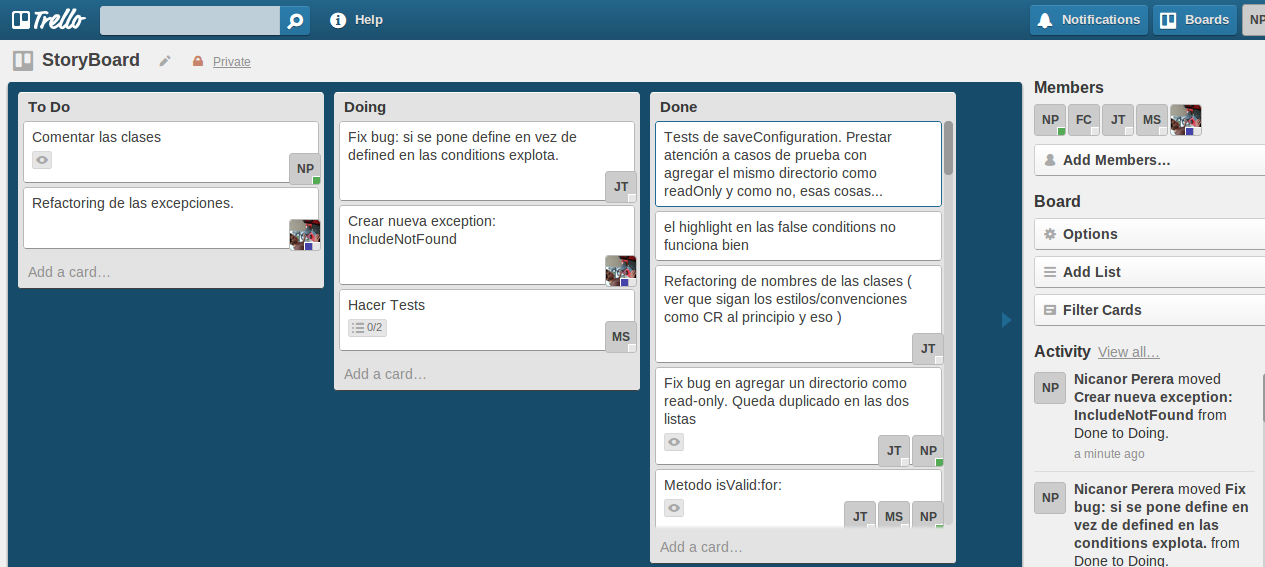
\includegraphics[scale=0.27]{images/trello.png}
    \caption{StoryBoard de trello}
\end{figure}

Trello facilitó todas las tareas de organización. Permitía que cada uno pueda elegir su tarea sin superponerse con la de el otro, podíamos ver lo que hacía cada uno en tiempo real y colaborar para llevar a cabo las tareas de la forma mas eficientemente posible. 

Adem\'as realizamos tests autom\'aticos para validar que las funcionalidades m\'as importantes se ejecuten correctamente.

\section{Frameworks y herramientas utilizadas}
El proyecto est\'a implementado en Smalltalk, utilizando el entorno de desarrollo VisualWorks. Para realizar los tests utilizamos el framework SUnit.

Smalltalk es un lenguaje de programaci\'on orientado a objetos y de tipado din\'amico y VisualWorks es una implementaci\'on multiplataforma de este lenguaje.

\section{Problema uno: Carga de archivos}

El primer paso para trabajar con CRefactory es seleccionar los archivos de c\'odigo C al cual se le va a aplicar el refactoring y las carpetas donde se encuentran los archivos de cabecera que incluyen dichos archivos (include directories).

Un archivo de cabecera es un archivo que el compilador incluye de forma automática al procesar algún otro archivo fuente. Estos archivos contienen normalmente una declaración directa de clases, subrutinas, variables u otros identificadores.

\subsection{Contexto}
La carga de archivos en la interfaz original funcionaba de la siguiente manera:

\begin{figure}[h!]
  \centering
    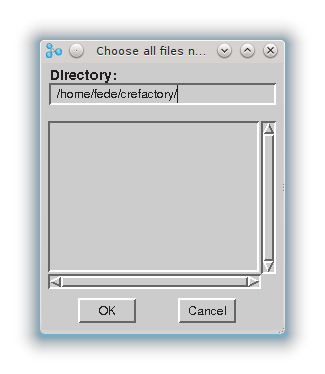
\includegraphics[scale=0.85]{images/codigo_original/carga.png}
    \caption{Carga de archivo original}
\end{figure}

Se deb\'ia escribir a mano el path absoluto hacia donde estaban los archivos. Esto era propenso a errores ya que se podían cometer errores de tipeo o incluso no recordar exactamente cual era dicho path.

Los path absolutos señalan la ubicación de un archivo o directorio desde el directorio raíz del sistema de archivos.

As\'i mismo el path inicial estaba escrito a mano (harcoded) con lo cual producía el siguiente error.

\begin{figure}[h!]
  \centering
    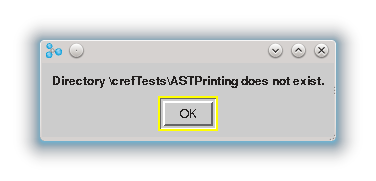
\includegraphics[scale=0.85]{images/codigo_original/error.png}
    \caption{Error }
\end{figure}

\subsection{Soluci\'on planteada}
El problema se solucion\'o agregando una ventana de exploraci\'on de archivos. Este permitió explorar el filesystem y seleccionar el archivo deseado. Ahora se podría seleccionar m\'as de uno al mismo tiempo.
Las ventajas de esta aproximaci\'on son que es menos propensa a errores y el usuario no necesita recordar el path absoluto.

A continuaci\'on mostramos un pantallazo de la visualizaci\'on de la nueva ventana de exploraci\'on de archivos:

\begin{figure}[h!]
  \centering
    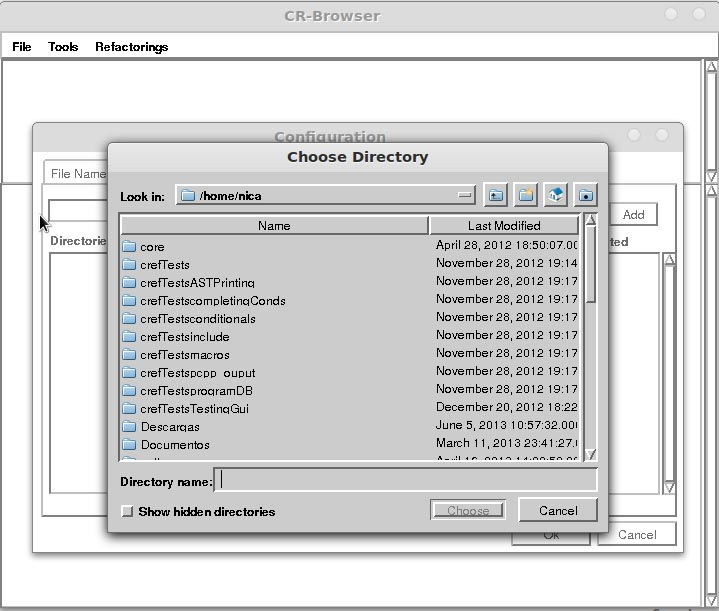
\includegraphics[scale=0.50]{images/codigo_modificado/seleccionar_directorio.jpg}
     \caption{Carga de archivo}
\end{figure}

\section{Problema dos: Nueva interfaz para la configuraci\'on}

\subsection{Contexto}
¿ C\'omo estaba la aplicacion ? ¿ Por qu\'e eso es un problema ?

\subsection{Soluci\'on planteada}
Cu\'al fue la soluci\'on al problema

\section{Problema tres: Manejo de excepciones}

El manejo de excepciones es una t\'ecnica de programaci\'on que permite controlar los errores ocasionados durante la ejecucici\'on del programa.
A continuaci\'on se detallan los problemas que presentaban la ausencia del manejo de estas en la interface de CRefactory y como fueron solucionados estos problemas.

\subsection{Contexto}
Ante un error de parseo la aplicación dejaba de funcionar. No había ningún tipo de manejo de excepciones. No encontrar un archivo de cabecera en los directorios incluidos significaba que el programa se cerrara abruptamente, sin ningún tipo de feedback para que el usuario pueda rastrear el error. Se hizo evidente la necesidad de que el usuario pudiera rastrear el error y corregirlo sin que falle la herramienta.

\begin{figure}[h!]
  \centering
    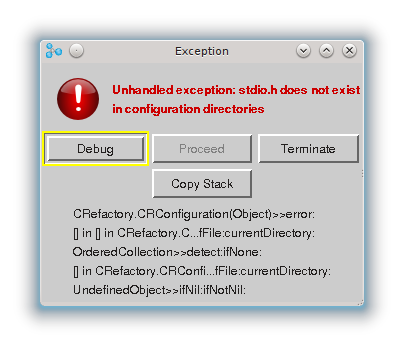
\includegraphics[scale=0.85]{images/codigo_original/error_header_no_agregado.png}
     \caption{Error por header no incluido}
\end{figure}

\subsection{Soluci\'on planteada}
Lo que se hizo en un principio fue implementar los manejadores para las excepciones. Por lo que cuando se produc\'ia una excepci\'on se mostraba una ventana con una descripci\'on del error. As\'i dandole feedback al usuario para que puediera corregir el error. Por ejemplo, cuando no se inclu\'ia el directorio donde buscar un header se mostraba una ventana advirtiendo del error y dandole al usuario la posibilidad de corregirlo agregando el directorio necesario en la ventana de configuraci\'on.

A continuaci\'on se visualiza como se mostraba el error luego de implementar el manejo de excepciones.

\begin{figure}[h!]
  \centering
    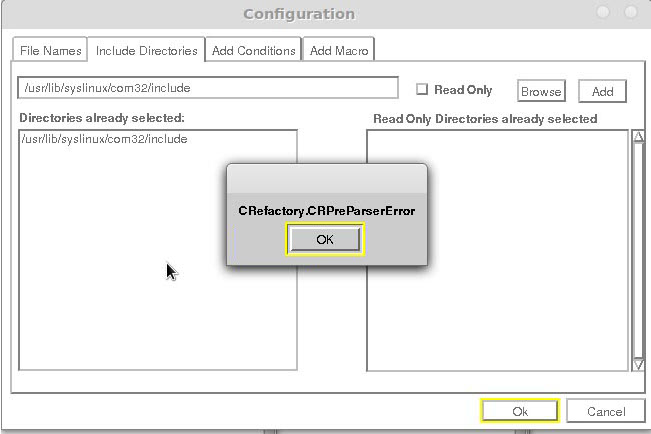
\includegraphics[scale=0.50]{images/codigo_modificado/error_header_no_encontrado_sin_view_error.jpg}
     \caption{Error por header no incluido}
\end{figure}

\section{Problema cuatro: Ventana de error}

Al ocurrir una exepci\'on no hab\'ia manera de que el usuario puediera tratarla. Se vi\'o la necesidad de visualizar el problema gr\'aficamente a trav\'es de una ventana de error

Una ventana es un \'area visual que contiene alg\'un tipo de interfaz de usuario, mostrando la salida y permitiendo la entrada de datos para los procesos en ejecuci\'on. Las ventanas pueden ser manipuladas con un puntero.

A continuaci\'on se explica como se trataba antes la excepci\'on, que problemas tra\'ia esto y como fueron solucionados.

\subsection{Contexto}
El problema de la soluci\'on planteada en el punto anterior es que no mostraba en que parte del c\'odigo fuente se produjo el error. Por lo tanto el usuario no siempre pod\'ia recuperarse totalmente.

\subsection{Soluci\'on planteada}
\'Esto llev\'o a reemplazar la ventana de notificaci\'on de error por una que diera la posibilidad de visualizar el c\'odigo fuente informando el error que se produjo. A continuación se muestra una imagen de la ventana mostrando el error.

\begin{figure}[h!]
  \centering
    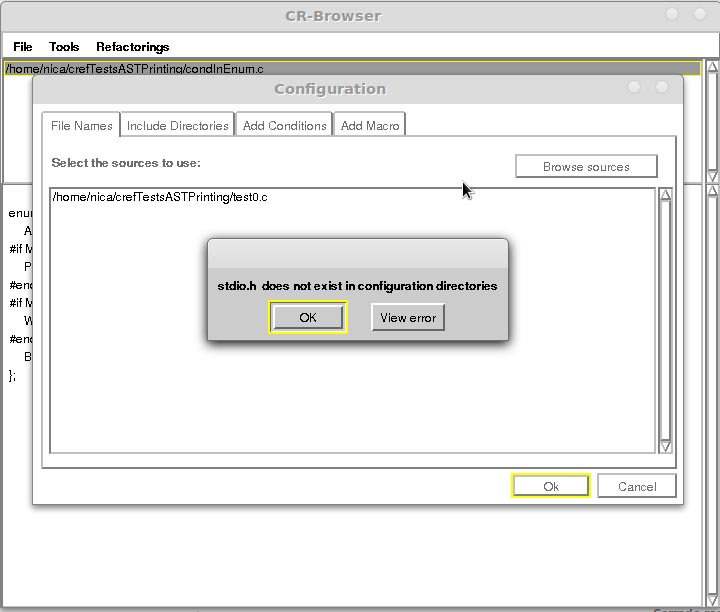
\includegraphics[scale=0.50]{images/codigo_modificado/error_header_no_encontrado.jpg}
     \caption{Error de header no encontrado}
\end{figure}

\section{Problema cinco: Highlight del error}

Cuando ocurre un error es útil conocer que linea o lineas de código son las que lo provocaron. Para poder identificar una porción de código, estuvimos de acuerdo en que sería muy útil contar con algún tipo de resaltado de texto. A continuación se explica cómo se mostraba el código antes, que problemas traía ésto y cómo fueron solucionados.

\subsection{Contexto}
Anteriormente, luego de un error se mostraba el c\'odigo pero no era claro que l\'ineas lo hab\'ian producido. Esto era un problema ya que la idea del manejo de excepciones no es solo identificar el error sino encontrar la manera de solucionarlo. Y muchas veces para solucionar un problema es necesario saber exactamente en que porci\'on del c\'odigo se origin\'o.

\subsection{Soluci\'on planteada}
El problema se solucion\'o implementando en la interfaz el resaltado de las l\'ineas donde se produjo el error. Gracias a \'esto el programador puede solucionar los errores con mucha mayor facilidad.

A continuaci\'on se visualiza el resaltado de un error.
\begin{figure}[h!]
  \centering
    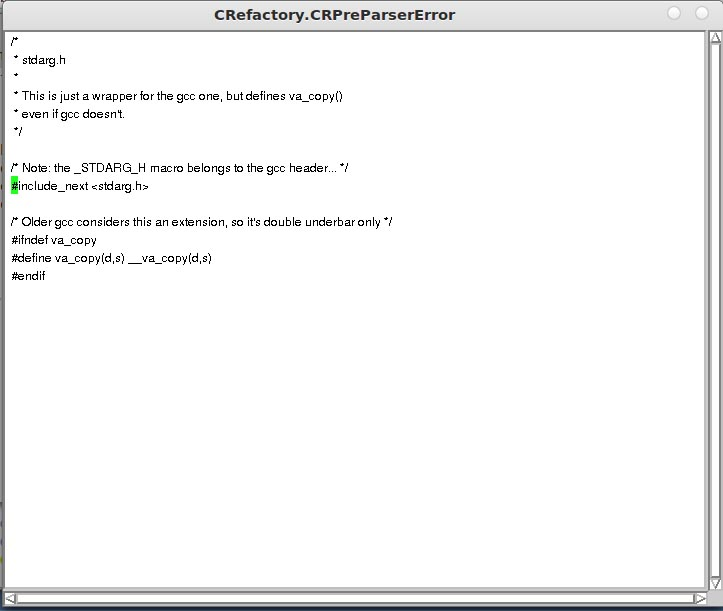
\includegraphics[scale=0.50]{images/codigo_modificado/highlight_preparser.jpg}
     \caption{Resaltado del error}
\end{figure}


\section{Instrucciones de instalaci\'on y uso}
En esta secci\'on se detallar\'an las instrucciones de instalaci\'on y uso de la herramienta.

\section{Minutas}
Durante el desarrollo del proyecto tuvimos varias reuniones con la Profesora, con la finalidad de conocer cu\'ales eran los requerimientos y mostrar el avance del proyecto. Cada vez que ten\'iamos una reuni\'on deb\'iamos tomar apuntes de lo que hab\'iamos hablado.

A continuaci\'on presentamos dichos apuntes o minutas:

\subsection{Reuni\'on del lunes 10/09}
La profesora nos di\'o una breve introducci\'on al proyecto y un vistazo general de c\'omo est\'a organizado. Nos explic\'o c\'omo estaba funcionando hasta ese momento. Aprendimos c\'omo cargar el proyecto dentro de visualworks y a realizar todas las configuraciones necesarias para el correcto funcionamiento de la aplicaci\'on.

Nos explic\'o c\'omo conectarnos al repositorio de la c\'atedra y c\'omo utilizar la herramienta de control de versiones.
Acordamos que nos enviar\'ia por correo electr\'onico los nombres de usuarios y contraseñas de cada integrante del grupo para acceder al repositorio.

Luego de \'esta introducci\'on al proyecto hablamos las funcionalidades que tendr\'iamos que implementar a lo largo de la cursada. Las m\'as importantes:

\begin{itemize}
  \item Mejorar el di\'alogo de carga de un archivo. Que sea por ejemplo como el de carga de parcels, haciendolo m\'as accesible al usuario.
  \item Poder especificar donde estan los directorios con los headers.
  \item Tener en cuenta las configuraciones que no se pueden parsear.
  \item Manejar las excepciones para que cuando hay una configuraci\'on inv\'alida muestre en el c\'odigo donde esta lo inv\'alido. 
\end{itemize}

Adem\'as se coment\'o que ser\'ia interesante como trabajo a futuro, posibilitar la creaci\'on autom\'atica de grafos de la inclusi\'on de archivos.

\subsection{Reuni\'on del lunes 17/09}
En \'esta reuni\'on la Profesora nos enseñ\'o c\'omo funcionaba el diálogo de carga de archivos. Anteriormente era necesario escribir el nombre de los archivos a incluir, lo cual hac\'ia tedioso el trabajo y ocurr\'ia que ante un error de tipeo no se encontrar\'ia el archivo y el programa cerrar\'ia abruptamente. 

Planteamos modificar el di\'alogo de carga de archivo para que permita explorar el file system. De esta manera ser\'ia m\'as f\'acil de utilizar y se solucionar\'ian los problemas.

\subsection{Reuni\'on del Jueves 18/10}
Para este momento ya hab\'iamos implementado la carga de archivos y directorios por medio de un File Browser, pero todav\'ia no era el ideal.

En esta reuni\'on se habl\'o con la profesora sobre la necesidad de marcar a algunos directorios como directorios de s\'olo lectura (Read Only).

Tambi\'en hablamos sobre la implementaci\'on de manejo de excepciones. En particular ocurr\'ia frecuentemente una excepci\'on al no incluir los directorios necesarios. Acordamos implementar el manejo de dicha excepci\'on.


Adem\'as comentamos los siguientes puntos:
\begin{itemize}
 \item Mejorar la secci\'on include Directory, para que se puedan agregar directamente.
 \item Bajar un ejemplo opensource en C para probar el funcionamiento.
 \item Prestar atenci\'on a preprocess y a FullNameOfFile.
\end{itemize}

\subsection{Reuni\'on del lunes 29/10}
En esta reuni\'on comenzamos a hablar sobre el tratamiento de excepciones en CRefactory. La profesora nos aconsejó que leamos la documentación del manejo de excepciones en Visual Works y que miraramos ejemplos en su código fuente para elegir la estrategia a utilizar.

Cuando se producía un error, CRefactory no indicaba cu\'al era el archivo que lo hab\'ia producido. Nos propusimos como objetivo que se pueda mostrar dicho archivo, y resaltar la l\'inea de c\'odigo en la cu\'al se produjo el error.

\subsection{Reuni\'on del 12/11}
Se hablaron los siguientes puntos:
\begin{itemize}
\item Que pasen los tests de CRefactory.
\item Si no puedo parsear una configuraci\'on, debo ponerla como condici\'on falsa.  El problema es que el error puede ocurrir en muchos lugares.
\item Debemos comenzar probando con el test19.c (el que tiene el \#ifdef\_cplusplus).
\end{itemize}

\subsection{Reuni\'on del 29/11}
Se hablaron los siguientes puntos:
\begin{itemize}
\item Cachear la excepci\'on al agregar False Conditions. 
\item Mirar en el preprocessor, en la linea: completeConditionalsFrom: OutputStream.
\end{itemize}

\section{Conclusiones}

\subsection{Logros alcanzados}
La nueva interfaz es pr\'actica para cargar archivos, directorios, macros y false conditions. Ahora se pueden cargar archivos de forma segura. En lugar de escribir el nombre del archivo o directorio se lo puede seleccionar entre los ya existentes. 

Ahora es posible acceder a funcionalidades que antes no se pod\'ian, como por ejemplo la posibilidad de agregar FalseConditions a la configuraci\'on para que no sean parseadas.

Cambiamos el diseño de la interfaz de manera que sea, a nuestro criterio, mucho m\'as amigable con el usuario.

Al dispararse una excepci\'on de parseo, la nueva interfaz ahora permite detectar la línea de código en la cual ocurrió.

\subsection{Valores obtenidos}
Trabajamos utilizando una metodología \'agil de tipo Scrum. Ésto nos permiti\'o tener una buena organizaci\'on. Ayud\'o al trabajo en equipo, optimiz\'o la eficiencia en la resoluci\'on de las tareas.

Comprendimos la importancia de realizar tests automatizados durante la programaci\'on. Si bien nos demor\'o implementar el c\'odigo de los tests, creemos que a la larga salimos beneficiados con respecto a la distribuci\'on del tiempo. Además saber que el programa segu\'ia funcionando nos daba mucha más seguridad al programar.

\subsection{Trabajo futuro}
En orden de conseguir que CRefactory sea una herramienta profesional que pueda competir con otros productos similares creemos que se debe soportar las siguientes caracter\'isticas:

\subsubsection{Coloreado de Sintaxis}
El coloreado de sintaxis es una caracter\'istica muy com\'un en los editores de texto modernos, y consiste en mostrar el c\'odigo fuente en diferentes colores con el objetivo de mejorar la legibilidad del c\'odigo para el programador.

\subsubsection{Localizaci\'on autom\'tica de c\'odigo refactorizable}
Actualmente, para realizar refactoring en el c\'odigo, el programador debe identificar el problema observando el c\'odigo. Creemos que ser\'ia buena idea implementar un algor\'itmo que sirva para localizar c\'odigo potencialmente refactorizable de manera autom\'atica.

\subsubsection{Integraci\'on con frameworks de testing}
Al hacer refactoring en el c\'odigo, debemos comprobar que el c\'odigo siga funcionando correctamente. Ser\'ia deseable que CRefactoring tenga integrados frameworks de testing para realizar el testeo del c\'odigo de forma autom\'atica.

\subsubsection{Personalizaci\'on del entorno}
Ser\'ia bueno otorgar a la interface cierta flexibilidad para poder adaptarse a las necesidades de cada usuario.


\subsubsection{Formateo autom\'atico de c\'odigo}
El formateo de c\'odigo es una herramienta que permite modificar el c\'odigo para que \'este se presente siguiendo convenciones de identaci\'on, espaciado y posicionamiento. \'Esto ayuda a que el c\'odigo sea m\'as f\'acil de leer, entender y mantener para el desarrollador.

Creemos que ser\'ia ideal que CRefactory cuente con una herramienta de formateo autom\'atico.


\subsubsection{Tabla de S\'imbolos}
Una tabla de s\'imbolos es una estructura de datos donde cada s\'imbolo en el c\'odigo fuente de un programa est\'a asociado con informaci\'on, como por ejemplo la ubicaci\'on, el tipo de datos y el \'ambito de cada variable.

Ser\'ia bueno poder ver la tabla de s\'imbolos.

\subsubsection{Grafo de dependencias}
Puede ser \'util visualizar las dependencias de los archivos. Ser\'ia interesante contar con una herramienta que realize grafos de inclusi\'on de archivos de forma autom\'atica.

\end{document}